\documentclass[14pt]{article}
\usepackage{geometry}                
\geometry{letterpaper}                   
\usepackage[bottom]{footmisc}
\usepackage{graphicx}
\usepackage{amssymb}
\usepackage{blindtext}
\usepackage{epstopdf}
\usepackage{braket}
\usepackage{float}
\usepackage[colorlinks,bookmarks=false,linkcolor=blue,urlcolor=blue]{hyperref}
\usepackage{natbib}
\usepackage{dirtytalk}
\usepackage{algorithmic}
\usepackage{mathtools}
\usepackage{amssymb, amsmath}
\usepackage[ruled,vlined,linesnumbered,noresetcount]{algorithm2e}
\usepackage{pdfpages}
\DeclareGraphicsRule{.tif}{png}{.png}{`convert #1 `dirname #1`/`basename #1 .tif`.png}
\providecommand{\reff}[1]{(\ref{#1})}
%\title{Title}
%\author{Anas Bachiri, Karlis Briedis}
%\date{date} 


\begin{document}



\thispagestyle{empty}

\begin{center}

\includegraphics[width=5cm]{img/ETHlogo.eps}

\bigskip


\bigskip


\bigskip


\LARGE{ 	Lecture with Computer Exercises:\\ }
\LARGE{ Modelling and Simulating Social Systems\\}

\bigskip

\bigskip

\small{Project Report}\\

\bigskip

\bigskip

\bigskip

\bigskip


\begin{tabular}{|c|}
\hline
\\
\textbf{\LARGE{The Impact of Network Topology}}\\
\textbf{\LARGE{on Banking Default Dynamics}}\\
\\
\hline
\end{tabular}
\bigskip

\bigskip

\bigskip

\LARGE{Anas Bachiri  \& K\={a}rlis M\={a}rti\c{n}\v{s} Briedis}



\bigskip

\bigskip

\bigskip

\bigskip

\bigskip

\bigskip

\bigskip

\bigskip

Z{\"u}rich\\
Dec 2018\\

\end{center}



\newpage


\includepdf[pages=-]{declaration_originality.pdf}

\newpage
\section*{Agreement for free-download}
\bigskip


\bigskip


\large We hereby agree to make our source code for this project freely available for download from the web pages of COSS. Furthermore, we assure that all source code is written by ourselves and is not violating any copyright restrictions.

\begin{center}

\bigskip


\bigskip


\begin{tabular}{@{}p{3.3cm}@{}p{6cm}@{}@{}p{6cm}@{}}
\begin{minipage}{3cm}
\pagenumbering{gobble}
\end{minipage}
&
\begin{minipage}{6cm}
\vspace{2mm} \large Anas Bachiri

 \vspace{\baselineskip}

\end{minipage}
&
\begin{minipage}{6cm}

\large Karlis Briedis

\end{minipage}
\end{tabular}


\end{center}

\newpage
\pagenumbering{gobble}
%%%%%%%%%%%%%%%%%%%%%%%%%%%%%%%%%%%%%%%

%%%%%%%%%% Table of content %%%%%%%%%%%%%%%%%

\tableofcontents
\pagenumbering{gobble}
\newpage
\pagenumbering{arabic}
\setcounter{page}{1}
%%%%%%%%%%%%%%%%%%%%%%%%%%%%%%%%%%%%%%%



\section{Abstract}
Systemic risk is of crucial importance when dealing with complex systems. In particular, financial networks are an important illustration of such systems. In this case, financial institutions interacts with each others respecting the graph structure of the underlying network. 
\\ Recent studies \cite{art2} have revealed the relevance of financial network structure in estimating systemic risk. It has also showed that the neglect of the graph topology is seriously underestimating the risk of default of the whole network.
\\ In this project, we address the issue of crisis propagation in a banking network. We construct first a banking system with some parameters, distribute the assets on the banks  and finally we simulate shocks in this financial network.
\\ This work investigate the general behaviour of crisis propagation in a financial network, and therefore provides some insights about reducing the systemic risk. For this, we will scan the parameters of the used model and describe the behaviour of the resilience of financial networks.
\vspace{65mm}

\section{Individual contributions}

% We collaborated equally on this project, and we had also to discuss several aspects of it.
% Karlis Briedis was responsible of the simulations and the generation of plots and figures, and Anas Bachiri provided the general approach to tackle the addressed problem and was responsible of writing the flash-talk and the final report.

We collaborated equally on this project, and we had regular meetings were discussed scientific papers we had studied on this topic and further direction of the project.
K\={a}rlis M\={a}rti\c{n}\v{s} Briedis was responsible for coding and writing subsection "Complex netowrk structure simulation", and Anas Bachiri provided the general approach to tackle the addressed problem and was responsible of writing the flash-talk and the final report and adapted the solution to observe dynamics in networks generated by the stochastic block model.

\section{Introduction and Motivations}

Systemic risk is the risk of failure of the whole system, or of the majority of its components. In a financial situation, this is equivalent to the risk of collapse of the whole financial network and therefore the collapse of the economy.
\\ One of the driving motivations of this work was the financial crisis 2008. The latter had dramatic consequences on the world's economy, it had affected also the GDP growth rates for several countries.

\begin{figure}[h]
\begin{center}
  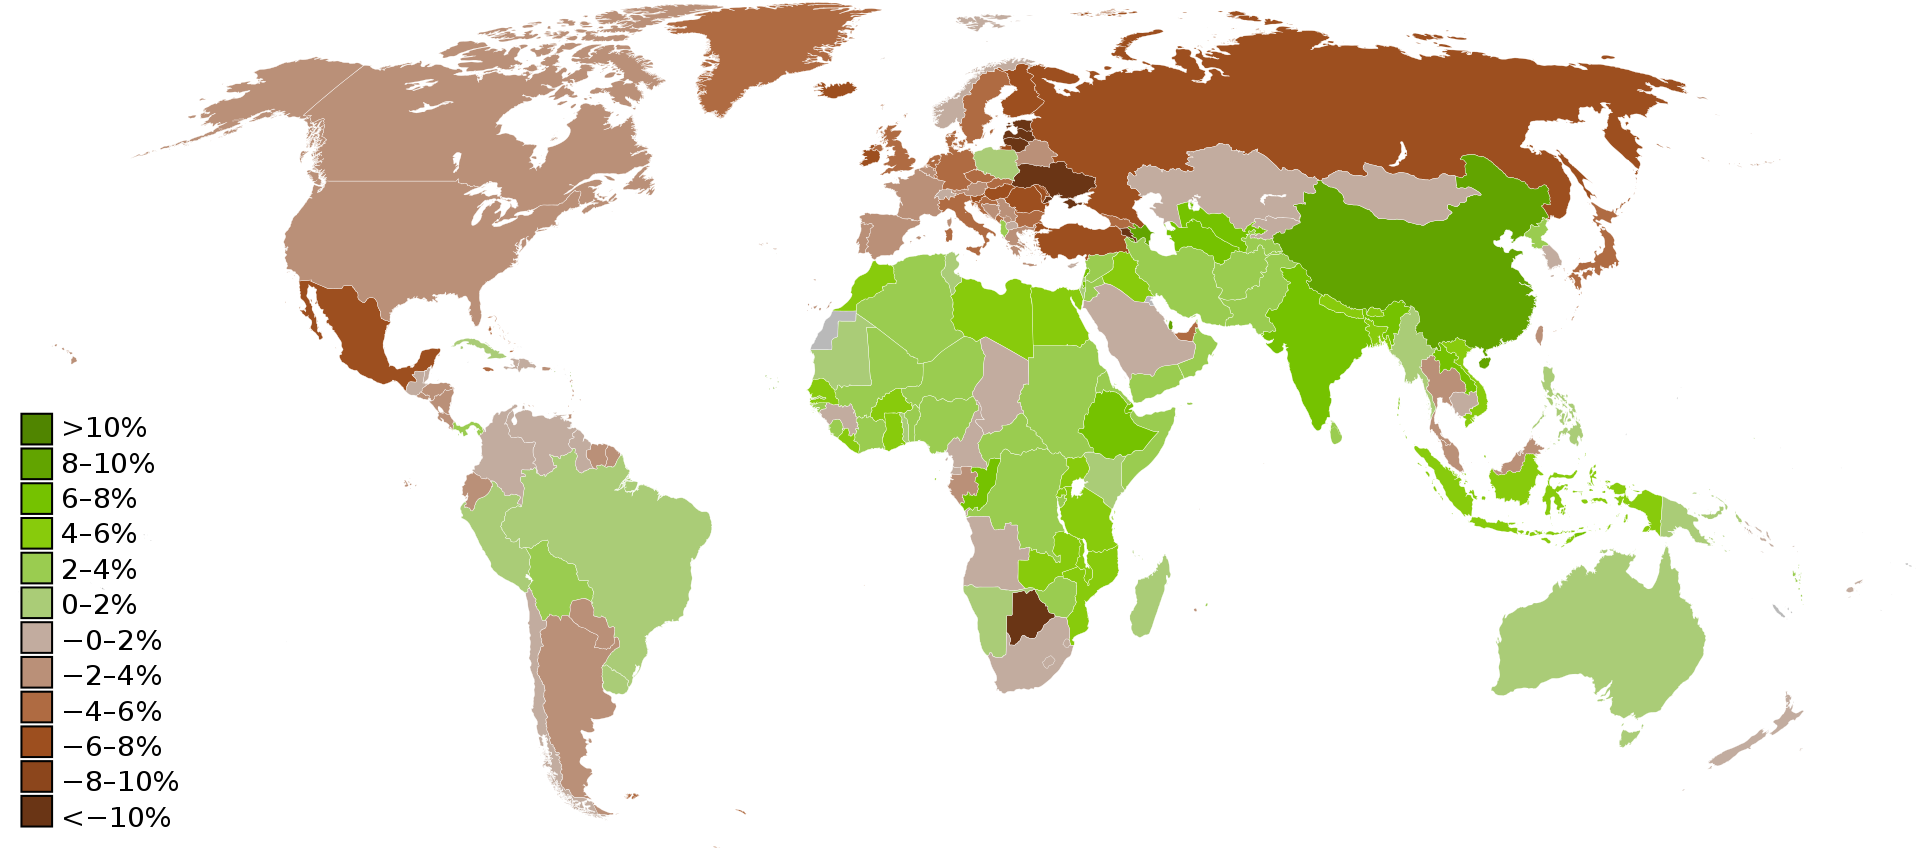
\includegraphics[width=0.98\linewidth]{img/fig1.png}
  \caption{Gross domestic product (GDP) growth rates during 2009\cite{Wiki}.}
  \label{fig:1}
  \end{center}
\end{figure}

This work was also motivated by our eager to learn how banking networks could be modelled, how contagion in networks is spread. And finally, to give some insights about what can be done in term of regulations to reduce the systemic risk of the banking networks.
\\ There are several mechanisms that can provoke systemic failure in a banking network. The first mechanism which will be focusing on is : financial relations or direct bilateral exposure between banks\cite{art1}. In fact, as we shall see later, having a small number of financial partners increases the risk of individual bank failure, \say{Since there are no partners to absorb the shock, the concerned bank will default}. 
\\Other causes of the systemic risk are the informational contagion and feedback effects.
\\In this work, We will also see the effects of level of capitalization of the banking network on the systemic risk and shock propagation.
\section{Theoretical foundations}
In this part we will shorty introduce relevant models and their theoretical construction, to establish a basis to the framework used to generate the banking system.
\subsection{The $G(n,p)$ model}
The $G(n,p)$ or the Erd{\"o}s-Renyi model refers to a method of constructing random graph that is analytically tractable. The model was introduced by Paul Erd{\"o}s and Alfred Renyi \cite{art3}, and it has two parameters $n$ and $p$.
\\The first parameter $n$ specifies the number of nodes $|V|$ of the graph $G=(V,E)$, while the second parameter $p$ refers to the rewiring probability, or the probability to link a couple of nodes $(v_i,v_j)$. Since the probability of linking two nodes is uniform, we obtain the following binomial degree distribution : $P(k) = {n-1\choose k}p^k(1-p)^{n-1-k}$.

\subsection{The Stochastic Block Model (SBM)}
In this part, we discuss the generation of graphs that has a \say{community like} structure. Such a model could be viewed as a generalization of the $G(n,p)$ model.
\\The SBM requires a set of parameters : $n$ is the number of nodes in the graph, a fixed number of $C$ blocks or communities, a community assignment vector $\Vec{z}$ of size n and values in ${0,...,C-1}$. The vector $\Vec{z}$ gives to each node a community label. Finally, the last parameter required by SBM is the \textbf{stochastic block matrix} $M \in \mathbf{R}^{CxC}$ which gives link probabilities between a pair of nodes $(v_i,v_j)$ with $z_{v_i}=k$ and $z_{v_j}=l$

\subsection{Complex network structure simulation}
\input{graph_generation.tex}

 \section{Description of the Model}
We have adopted the framework introduced in \cite{art1} to perform this benchmark to study the network resilience to financial crisis. To begin with, we start with the construction of the banking network. 
\\Due to the lack of data on the structure of such banking networks, we are going to adopt a probabilistic methods to generate such networks. There are several methods and models to generate networks, one important example is the Erd{\"o}s-Renyi graph $G(n,p)$, which generates a network $G=(V,E)$ with $n$ nodes : $|V|=n$, and the links are generated randomly between a pair of nodes with  probability $p$. In our case, the links created are directed and the probability is uniform for both directions.

\begin{figure}[h]
    \centering
  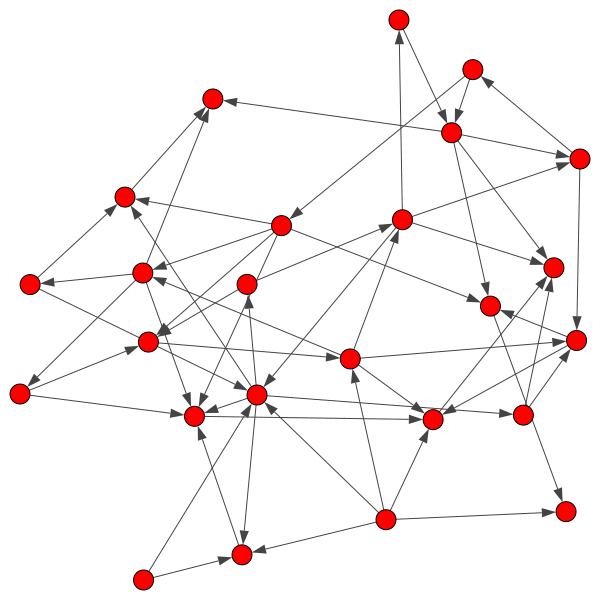
\includegraphics[width=0.5\linewidth]{img/fig2.png}
  \caption{An example of a directed network constructed with the $G(n,p)$ model with $n=25$ and $p=0.2$.}
  \label{fig:2}
\end{figure}
Considering that every node in fig.\reff{fig:2} is a bank, a directed edge represents the lending relationship between two banks.
\\Having built the network, we will now distribute the assets in this network. Such a task requires to fill the individual banks balance sheets consistently with the bank level and the aggregate balance sheet identities. We follow the same notation adopted in \cite{art1}, and capital characters will denote variable at the aggregated level.
\vspace{25mm}
\\Here we define the \textbf{parameters} used in the model :
\begin{itemize}
\item \textbf{A} : Total/aggregated assets of the banking system
\item \textbf{E} : Total/aggregated external assets of the banking
system  
\item \textbf{I} : Total/aggregated internal assets of the banking
system  
\item \textbf{Z} : Total number of links $|E|$ in the banking network
\item $\boldsymbol{\beta}$ : fraction of external assets $\beta = \frac{E}{A}$
\item $\boldsymbol{\theta}$ : percentage of inter-bank assets $\theta = 1-\beta$
\item $\boldsymbol{\gamma}$ : Net worth as percentage of total assets 
\end{itemize}
Note that each bank is also characterized by a set of parameters : $a_i$ denotes an individual bank assets, $e_i$ denotes external assets borrowing  and $i_i$ denotes inter-bank assets. Thus we have : $a_i = e_i + i_i$. Let $l_i$, $c_i$, $b_i$ and $d_i$ denotes respectively the individual liabilities, net worth, inter-bank borrowing and finally the customer deposit. We mention also that the aggregated assets satisfies the following rule : $\boldsymbol{A}=\boldsymbol{E} + \boldsymbol{I}$.
\\
\\In this part, we show how to assign numerical values to individual bank parameters $a_i$, $l_i$, $c_i$, $b_i$, $e_i$ and $d_i$ respecting the aggregate values of total internal \textbf{I} and external assets \textbf{E}. We will also how to model the shock spread.

\begin{minipage}[t]{5cm}
  \vspace{0pt}  
  \begin{algorithm}[H]
    \caption{Algorithm distributing assets according to the aggregated values  }
    \label{alg:1}
    \begin{algorithmic}
\STATE $w \gets \frac{\boldsymbol{I}}{Z}$
\FOR{i $\in [1,n]$}
\STATE $i_i \gets w \sum_{j=1}^n A_{ij}$
\STATE $b_i \gets w \sum_{j=1}^n A_{ji}$
\STATE $\Tilde{e}_i \gets max(b_i-i_i , 0)$
\ENDFOR
\FOR{i $\in [1,n]$}
\STATE $e_i \gets \Tilde{e}_i + [(E- \sum_{l=1}^n \Tilde{e}_i)/n]$ 
\STATE $a_i \gets e_i + i_i$ 
\STATE $c_i \gets \gamma a_i $ 
\STATE $d_i \gets a_i - c_i -b_i$ 
\ENDFOR
\end{algorithmic}
\end{algorithm}
\end{minipage}%
\begin{minipage}[t]{5cm}
  \vspace{0pt}
  \begin{algorithm}[H]
    \caption{Algorithm of shocks and shock transmission }
    \label{alg:2}
    \begin{algorithmic}
\STATE Let $s_i$ be the size of initial shock
\IF{$s_i > c_i$} 
\STATE the bank $i$ defaults
\ENDIF
\IF{$s_i - c_i - b_i \leq 0$} 
\STATE creditor banks lose $(s_i-c_i)$ distributed equally
\ELSE
\STATE Depositor banks lose $s_i-c_i-b_i$
\ENDIF

\end{algorithmic}
  \end{algorithm}
\end{minipage}%
\\Note that for the model, there are only five independent parameters which are scanned. In our case, these parameters are : $(\gamma , \theta, p , N,E)$. The first algorithm \reff{alg:1} shows how to assign individual bank values respecting the aggregated amount of internal and external assets, while the second algorithm \reff{alg:2} is for shock simulation.


\section{Implementation}
This program was implemented in python, and we used libraries such as : $iGraph$ library to generate Erd{\"o}s-Renyi networks $G(n,p)$, the $Matplot$ library to generate plots and figures. And other python libraries were used such as $Numpy$ to manipulate vectors and matrices. It is also possible to find our code in a GitHub repository \cite{git}.
\\We have first investigated the behaviour obtained in the paper \cite{art1}. For this, we have used the following benchmark values for the model parameters :
\begin{equation*}
    (\gamma , \theta, p , N,E) = ([0,0.1], 0.2, 0.2, 25, 100\,000)
\end{equation*}
The numerical value of $\gamma$ is scanned from $0$ to $0.1$, while the other parameters are set in fix values. 
\\We start by analyzing the resilience of the banking system and how is it affected by the net worth $\gamma$. Then we will study the effects of connectivity on system's resilience, and this is done by changing the probability p of the $G(n,p)$ model. Other questions may be also addressed concerning the network robustness, for example how the latter changes with the percentage of internal assets.
\\ Other parts of the implementation will be performing simulations on different network structures. The most important structures will be \say{The community like structure in networks}. This is analyzed to understand how does crisis propagates in an international financial network scenario. In this case, we can imagine that every \say{community}/cluster of nodes form the set of banks in some country, where they tend to connect heavily with each others, and have also few other connection with different other clusters \say{Banks in different countries}. We will be studying the same resilience properties in this international network situation.
\section{Simulation Results and Discussion}
\subsection{Percentage net worth and contagion}
The first simulation we perform is to count the number of defaults for every value of net worth percentage $\gamma$ scanned. 
\begin{figure}[h]
    \centering
  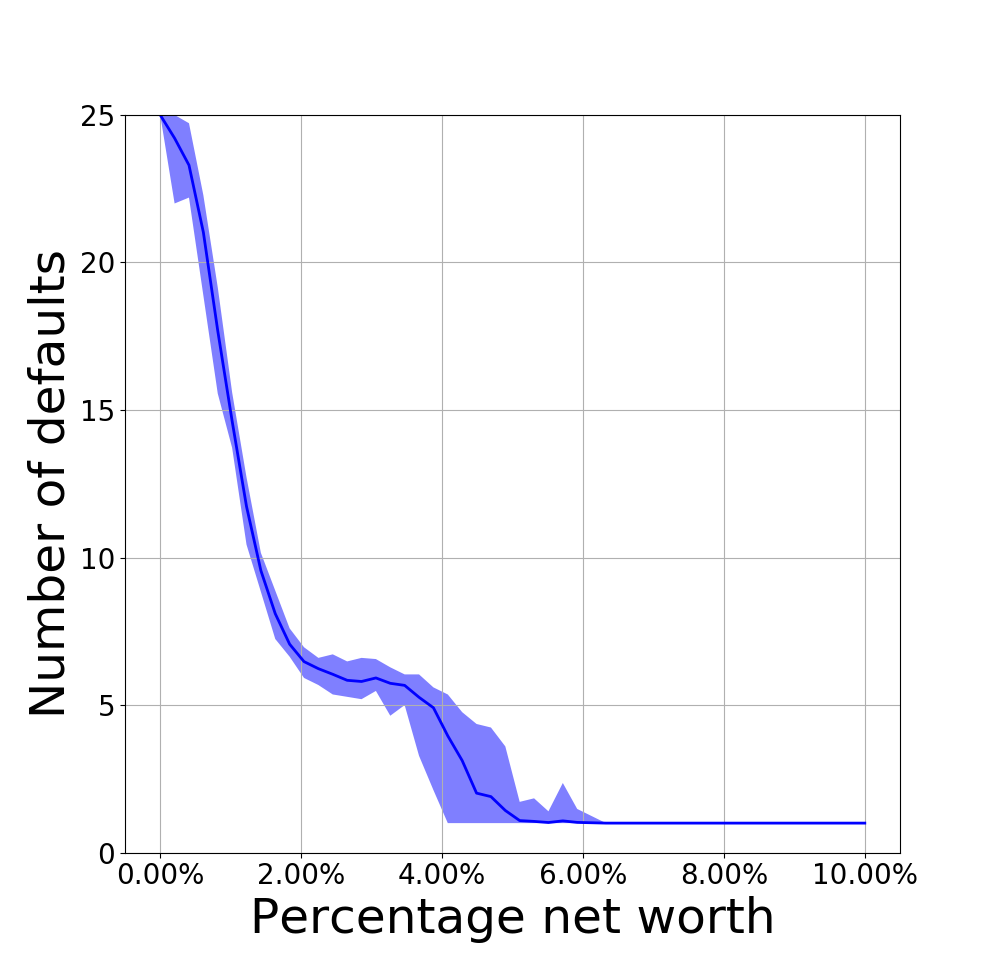
\includegraphics[width=0.6\linewidth]{img/Figure_3zbi.png}
  \caption{The effect of percentage net worth $\gamma$ on the number of defaults.}
  \label{fig:3}
\end{figure}
This is an evaluation method for the network resilience and how it is affected by the parameter $\gamma$. The results in figure \reff{fig:3} show that the number of defaults in the banking network decreases with the percentage of net-worth. In fact, as we mentioned previously, the net worth $c_i$ serves as a damping factor to the \say{financial shock}. The biggest the net worth, the more robust the bank is. Note also the three regimes obtained in the figure \reff{fig:3}:
\\First, there is a fast decreases in the number of defaults for $\gamma$ in the interval 
$[0,2]$\%. Second, a constant regime of the number of defaults for $\gamma \in [2,3.5]$, and in this part the number of defaults remains at $5$ defaulted banks. Finally, there is another decrease for $\gamma \in [3.5,6]$ and after that the the number of defaults remains the same after $\gamma = 6 \%$. The first fast decrease of defaulting banks could be explained by the  increase of $c_i$, this prevent the shock to propagate in the whole network. While the constant regime could be explained by the fact that the shock propagates only in the first neighbours of the initial shocked bank. Note that the defaulting banks stays constant around $6$, this value in fact could be obtained if we approximate the neighborhood of a node by the mean degree $\braket{k}=np$ for the $G(n,p)$ model. In our case $n=25$, $p=0.2$ leads to $\braket{k}=5$ plus the initial shocked bank, which explains the result \reff{fig:3} obtained.
\subsection{Connectivity and contagion}
Another analysis done concerning the effects of connectivity on network resilience. As we have mentioned before, the connectivity has two different effects. A high connectivity means that the shock can be easily absorbed by the network, since the loss of the shocked bank will be shared by its neighbours. But at the same time, high connectivity means that the shock could propagate easily in the network.

\begin{figure}[h]
    \centering
  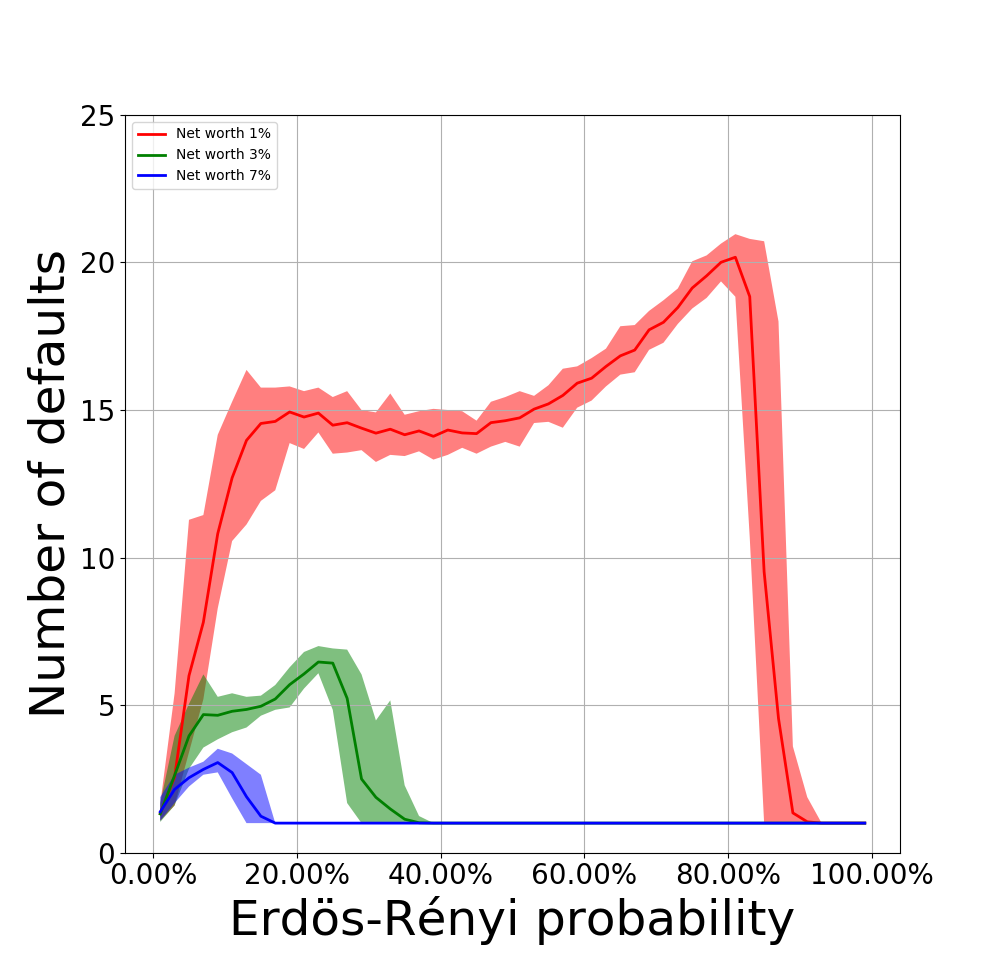
\includegraphics[width=0.6\linewidth]{img/fig4.png}
  \caption{The effect of connectivity on the number of defaults for different net-worth values $\gamma$.}
  \label{fig:4}
\end{figure}

The figure \reff{fig:4} is obtained by scanning the connectivity parameters p of the $G(n,p)$ model, and performing the shocks. 
This provides us with an idea about how connectivity and net-worth affect the spread of crisis. 
\\As we can see in figure \reff{fig:4}, the banks resilience is very sensitive to the parameter $\gamma$. For very low values of the net-worth percentage, the number defaulting banks is significantly high. Since there is no enough net-worth to absorb the shock, the latter is easily transmitted in the network. Note also that the graphs in \reff{fig:4} have a similar shape, the contagion spread is remarkably fast at the beginning, after that it remains constant, increase after that to finally decrease. This underlines the fact that there is no \say{general} rule we can follow, but what we can learn about this is the following : In case of a relatively high value of the net-worth percentage $\gamma \geq 7 \%$, a bank should be connected to $20\%$ of the other banks in the network to avoid systemic failure. For the case of very low net-worth percentage, banks should not be very connected to each other.
\subsection{Percentage inter-bank assets and contagion}
Other aspects of the network resilience were investigated, such as the effects of the percentage inter-bank assets on the number of defaults.
\begin{figure}[H]
    \centering
  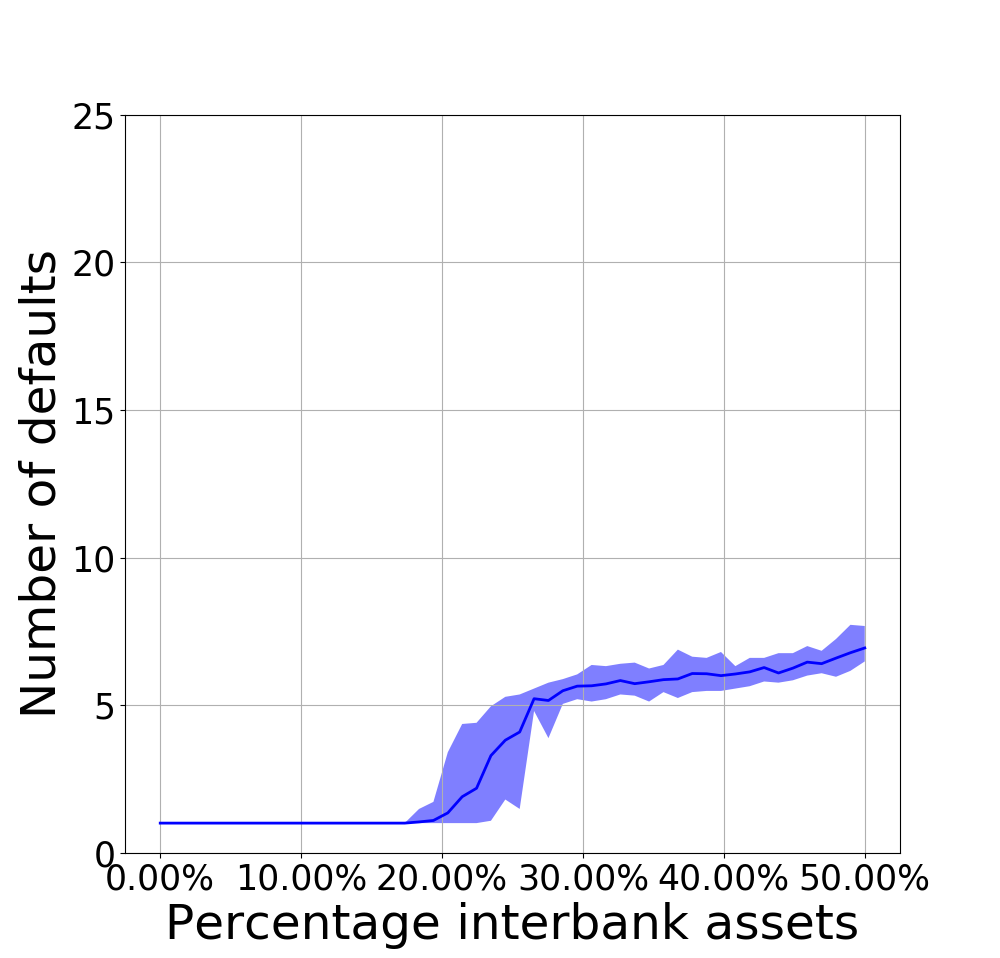
\includegraphics[width=0.6\linewidth]{img/fig5.png}
  \caption{The effect of percentage inter-bank assets $\theta$ on the number of defaults.}
  \label{fig:5}
\end{figure}
By maintaining the size of the external assets \textbf{E} constant, and by increasing the fraction of inter-bank assets. Intuitively, this means an increase in the size of lending in the network. Since we know from the previous sections that the inter-bank borrowing $b_i$ is proportional to $w = \frac{\boldsymbol{I}}{Z}$, and $Z$ being the total number of connections in the network.  We mention also that there are two opposite driving forces of the inter-bank assets percentage on the system's resilience. On the one hand, the bigger the size of lending in the network, the easier the transmission of an initial shock. On the other hand, increasing the fraction of inter-bank assets, means an increase in the total net worth, and therefore the capacity of the network to absorb shocks.
\\Effectively as we can see in figure \reff{fig:5}, there are no contagion effects for small values of percentage inter-bank assets, this is due to the absorption of \say{shocks} by customer deposits $d_i$. Besides, the loss level is also very so it is easily absorbed by banks net worth.

\subsection{Clustering coefficient and network resilience}

In this section we are going to study how network resilience is effected by the clustering coefficient of the network.
\begin{figure}[H]
    \centering
  \includegraphics[width=0.6\linewidth]{img/clustering.png}
  \caption{The effect of the clustering coefficient on the number of defaults.}
  \label{fig:clust}
\end{figure}
In this part, we use complex network structure simulation discussed above to generate random graphs respecting an average clustering coefficient. 
\\ The results obtained in figure \reff{fig:clust} have an extremely noisy character for very low values of the net worth. This property could be explained by the fact that for low values of $\gamma$, the number of defaults depends a lot on the graphical topology. In such a regime, network effects becomes extremely important, and this suggests that in the low damping case, it is quiet challenging to  estimate the number of defaults without considering the full network topology. Note also that the mean value has a decreasing trend, since the clustering in linked to connectivity. For high values of connectivity, we recover the same behaviour obtained for $G(n,p)$ graphs in figure \reff{fig:4}.

\subsection{International banking network}
After reproducing the results obtained in \cite{art1}, and obtaining the same results. In this section, we will extend the study to a different class of graphs.
\\We consider a scenario where the banks belong to different countries. In this case, each country has a specific number of banks, and banks within the same country are highly connected to each others compared to banks of different countries. By this, we model an international banking network, where lots of banks of a country are connected to each other, and only few of them have connections with \say{foreign} banks.
\begin{figure}[H]
    \centering
  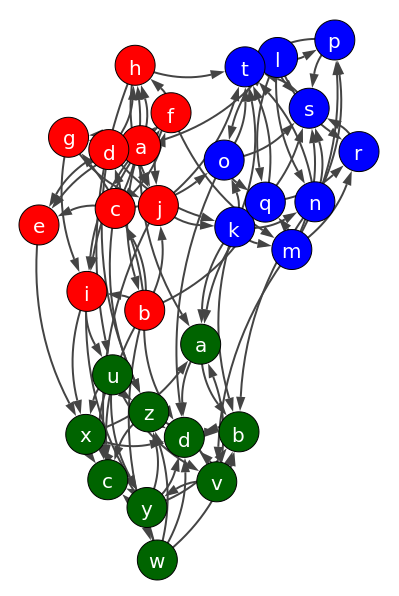
\includegraphics[width=0.35\linewidth]{img/fig6.png}
  \caption{Illustrative example of a $3$-communities network of $30$ Nodes.}
  \label{fig:6}
\end{figure}

These kind of networks are generated by the \textbf{Stochastic Block Model} discussed before. An illustrative example of such a network is given in figure \reff{fig:6}.
\\The community-like graphs used in the simulations have the following parameters : $n=75$ nodes, number of communities $C = 3$ and finally we have used two stochastic block matrices $M_1$ and $M_2$ :
\[ M_1 =\left( \begin{array}{ccc}
0.4 & 0.1 & 0.1 \\
0.1 & 0.4 & 0.1 \\
0.1 & 0.1 & 0.4
\end{array} \right)\>
% \
\> \;\; \; \; M_2 = \left( \begin{array}{ccc}
0.65 & 0.1 & 0.1 \\
0.1 & 0.65 & 0.1 \\
0.1 & 0.1 & 0.65
\end{array} \right)
\]
Note that the matrices $M_{1,2}$ are symmetric and their diagonal terms are higher than the non-diagonal ones. This translates to a case where each country establishes financial relationships with the other countries without any preference. Besides, the diagonal terms refers to the probability to create links within the same \say{country}. The non-diagonal terms are the probabilities to connect to banks in a different country.
\begin{figure}[!htb]
\minipage{0.32\textwidth}
  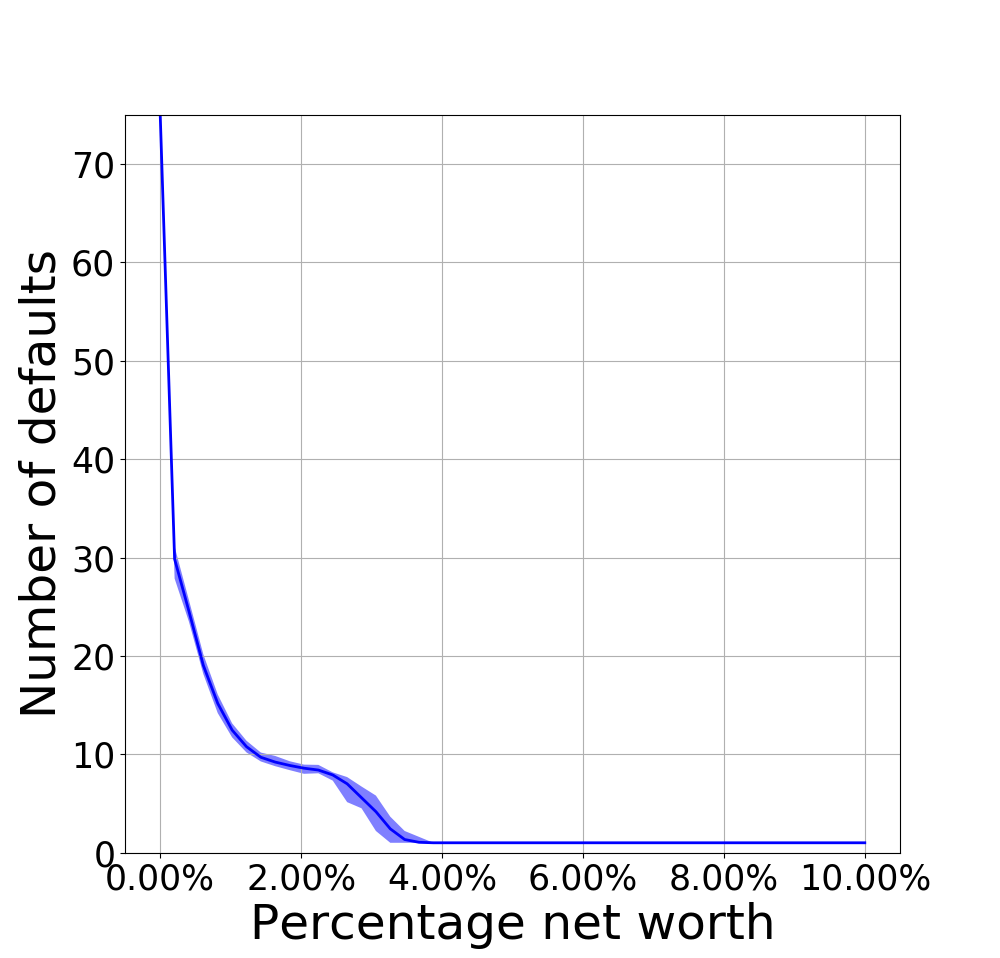
\includegraphics[width=\linewidth]{Figure_1N75pin40pex10.png}
  \caption{Simulation with SBN with $M_1$}\label{fig:7}
\endminipage\hfill
\minipage{0.32\textwidth}
  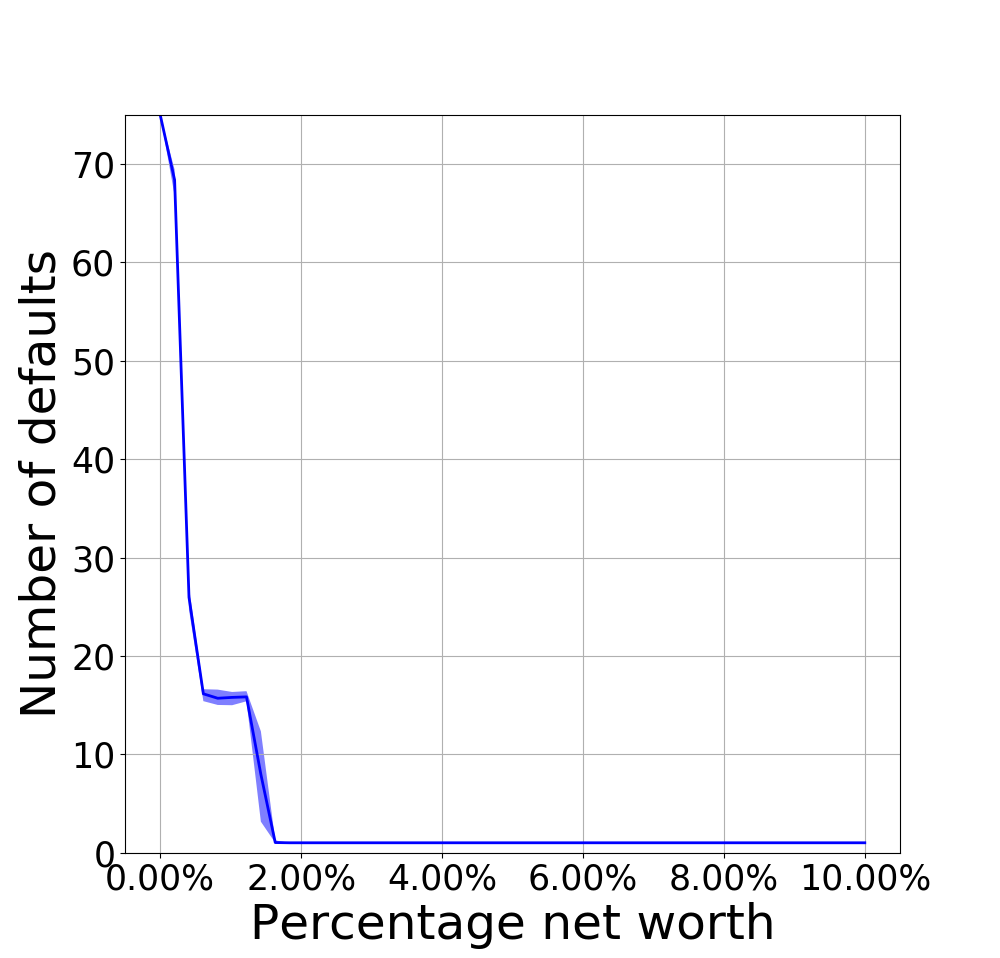
\includegraphics[width=\linewidth]{Figure_1_N75.png}
  \caption{Simulation with $G(n,p)$ model}\label{fig:8}
\endminipage\hfill
\minipage{0.32\textwidth}%
  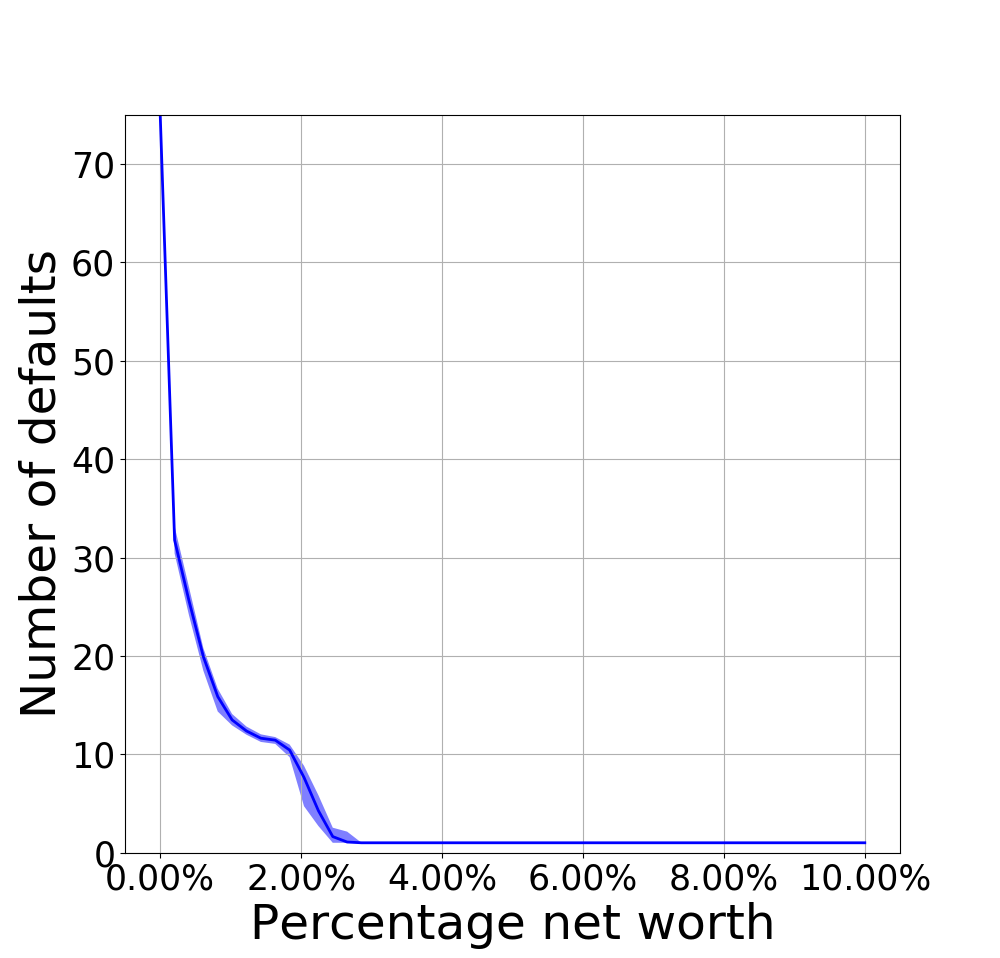
\includegraphics[width=\linewidth]{Figure_1N75pin65pext1.png}
  \caption{Simulation with SBN with $M_2$}\label{fig:9}
\endminipage
\end{figure}
We have also performed a simulation using the $G(n,p)$ model, using $n=75$ and $p=0.2$, and use this simulation as a ground truth to compare the difference between the \say{National and international} cases.
\\ The results of simulations in figures (\ref{fig:7},\ref{fig:8},\ref{fig:9}) shows some interesting behaviours. Note that for the first simulation using the stochastic block matrix $M_1$, with diagonal probability $p=0.4$, we observe that the number of default requires a percentage net worth $\gamma$ of $4\%$  to attain its minimal value. This value is about twice of the value required in a \say{national} or single country situation : In  the figure \reff{fig:8}, the number of defaults is minimal already at percentage $\gamma$ of $2 \%$. We stress also that in the $G(n,p)$ case, the \say{constant} regime of the function is close to $16$ defaulting banks. This number could be explained as before by the mean degree of the $G(n,p)$ model, which is in our case $\braket{k}=15$. 
\\ For the last figure \reff{fig:9}, we see that the number of defaults reaches the minimum slightly above $\gamma=2\%$, we also see that the curve is broader than result obtained using $M_1$. In fact, the simulation obtained using $M_2$ could be viewed as a middle case between the previous results of $G(n,p)$ model and SBM using $M_1$. 
\\ In the single country situation, the number of defaults decreases very fast and the minimum percentage net worth required in such a network is less than the one required in an international situation. If banks withing the same country are not highly connected -case of $M_1$-, the defaulting number curve is broadened, and banks need to have higher net worth percentage to dampen shock effects. For higher connected banks -case of $M_2$-, the curve is less broad, but still a higher percentage net worth is required compared to the single country situation.
\section{Summary and Outlook}
This work addressed several crucial points on financial networks and crisis. First, it showed the importance of network structures and network effects. We are also able to successfully reproduce the work done in \cite{art1}, and generalize it to other graph topologies, corresponding to both random and real world networks.
\\ Despite data scarce, we managed to adopt a general investigative approach to understand the effect of network topology on system's resilience. And in the case of banking networks, we have showed that the network robustness is sensitive to the net worth percentage $\gamma$. The results suggested also that $\gamma$ should be at least $5\%$ to reduce systemic risk.
\\ Other important outcomes of this work was to show that there is no general recipe to reduce systemic risk using only connectivity, or if we ignore the net worth value $\gamma$. In fact, network connectivity can at the same time foster and damp financial shocks. 
\\ The analysis of the percentage inter-bank assets showed that for values of $\theta$ starting from $20\%$, could lead to a higher number of defaulting banks. And therefore, banks should have at least $80\$$ of their assets outside the network. 
\\ In the international bank network scenario, we have seen that connecting to banks from different countries could increase the systemic risk. In this situation, the network is more resistant to shocks if banks within the same country are highly connected. This is also equivalent to say that if a bank want to establish international relationships, its percentage net worth $\gamma$ should be high. This goes in hand with the fact that only \say{important} banks which have international relationships.
\\Conserning the effects of average clustering coefficient, the obtained results had high variance, a characteristic property in real world networks. This actually can show the limiting part of using random models can have, real world networks can introduce noise in the observed quantities, and make predictions hard to make. This part also allowed us to check for a second time the sensitivity of the network resilience to the net worth percentage. 
\\Finally, this work was very important to understand how to model banks and financial shocks, there are also several points in which we could extend this work. One of them is to investigate the behaviour of the stochastic block model but for an asymmetric situation. A scenario where countries that are \say{close to each other} tend to have more connections than other countries, it is also possible to check the behaviour by scanning the entries of the stochastic block matrix  by constraining graphs to other real world properties, and finally by considering other important aspects like temporal interactions in the graph.
\bibliographystyle{unsrt}
\bibliography{bibliography}




\end{document}  



 
